\documentclass{article}
\usepackage[utf8]{inputenc}
\usepackage{hyperref}
\usepackage{graphicx}
\usepackage{listings}
\usepackage{geometry}
\geometry{margin=1in}

\title{Structured Session Engineering and the FLAT Methodology\\\large A Deterministic Framework for Large-Scale AI-Augmented Software Development}
\author{Mark Bunds + ChatGPT}
\date{April 2025}

\begin{document}

\maketitle

\begin{abstract}
Aurora is a modular reflex control framework designed to interact with AI systems through browser GUIs, enabling deterministic, stateful, and reproducible development workflows. This paper introduces Structured Session Engineering (SSE) and the File-based Logic Assembly Tree (FLAT) methodology — a layered architecture that overcomes the limitations of stateless LLM prompting by combining modular file tracking with persistent semantic memory scaffolds. Through browser-based reflex loops, Aurora enables prompt injection, DOM response capture, and modular logic restoration without the use of APIs.
\end{abstract}

\section{Introduction}
Recent advances in AI language models have made them viable as programming partners. However, the lack of persistence and state across sessions limits their utility in large-scale, modular software development. The Aurora project addresses these limitations by introducing Structured Session Engineering (SSE) and the File-based Logic Assembly Tree (FLAT). This paper documents the architecture, implementation, and experimental results of these methods.

\section{Background}
The FLAT methodology originated during development of the OpenSIM DCS system and matured through its application in the Aurora project. Aurora evolved from a reflexive wrapper around ChatGPT into a standalone system capable of session continuity, modular prompt injection, and autonomous response evaluation via browser interaction.

\section{System Architecture}
\subsection{FLAT (File-based Logic Assembly Tree)}
FLAT is a non-hierarchical, file-based tracking method for organizing modular Python code, session logs, test records, and architectural decisions. All sessions and modules are registered in flat text files (e.g., \texttt{MASTER\_INDEX.txt}, \texttt{MAGIC\_BUSES.txt}), which serve as traceable metadata containers.

\subsection{SSE (Structured Session Engineering)}
SSE formalizes the structure of AI interaction sessions using a trunk-branch-leaf metaphor. Each branch corresponds to a development or planning goal, and all code, commentary, and outcomes are recorded.

\subsection{Magic Buses}
Aurora’s internal pub/sub layer, known as “magic buses,” facilitates decoupled communication between subsystems and the AI agent. These include \texttt{edit\_bus}, \texttt{control\_bus}, \texttt{diagnostic\_bus}, and \texttt{interrupt\_bus}, among others.

\begin{figure}[h!]
\centering
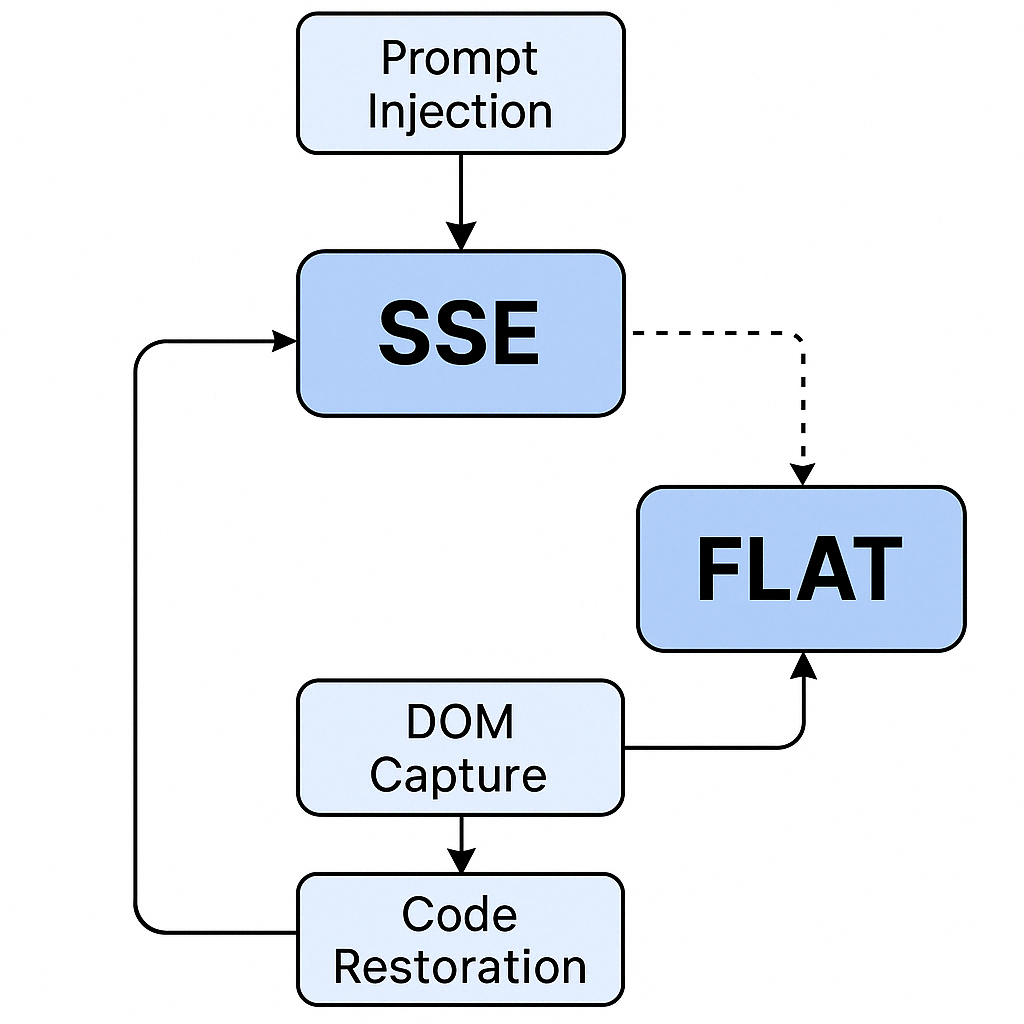
\includegraphics[width=0.95\textwidth]{graphics/aurora_reflex_flow.png}
\caption{Aurora Reflex Architecture: Prompt submission, DOM capture, and modular logic regeneration in a closed loop.}
\label{fig:aurora-flow}
\end{figure}

\section{Implementation}
The core modules are divided into \texttt{core/}, \texttt{web/}, \texttt{utils/}, and \texttt{tests/}. 

\begin{itemize}
  \item \texttt{session\_driver.py} launches browser sessions and injects prompts.
  \item \texttt{element\_mapper.py} enables DOM-to-logic mapping.
  \item \texttt{code\_restorer.py}, \texttt{code\_sanitizer.py}, and \texttt{code\_formatter.py} reconstruct flattened code into executable Python.
\end{itemize}

\section{Results}
A series of milestone logs captured Aurora’s successful interaction with the ChatGPT GUI:

\begin{itemize}
  \item Prompt injection and DOM response capture were achieved without API use.
  \item Flattened code blocks were successfully restored via the reflexive parsing pipeline.
  \item GUI-based control allowed Aurora to autonomously test, capture, and structure LLM outputs.
\end{itemize}

\section{Discussion}
Aurora demonstrates the viability of combining GUI-based reflex loops with flat-file session tracking to achieve deterministic AI-assisted development. SSE allows modular session segmentation and state restoration, while FLAT enables traceable history and reproducibility. Together, they constitute a scalable foundation for AI-augmented software engineering.

\section{Conclusion and Future Work}
Aurora represents a working prototype of an AI reflex agent capable of structured prompting, semantic memory scaffolding, and modular code restoration. Future extensions include:

\begin{itemize}
  \item Integration of local LLMs
  \item Enabling dual-channel interaction (e.g., GUI + API fallback)
  \item Expanded file agency and permission routing
\end{itemize}

\appendix
\section{Example Output: Restored Code Block}
\begin{lstlisting}[language=Python]
class YAMLConfigValidator:
    REQUIRED_FIELDS = ['project_name', 'version', 'author', 'settings']
    def __init__(self, config_path):
        self.config_path = config_path
        self.config_data = None
        self.errors = []
    def load_config(self):
        if not os.path.exists(self.config_path):
            raise FileNotFoundError(f"Config file not found: {self.config_path}")
        with open(self.config_path, 'r') as f:
            self.config_data = yaml.safe_load(f)
    def validate(self):
        for field in self.REQUIRED_FIELDS:
            if field not in self.config_data:
                self.errors.append(f"Missing field: {field}")
        return not self.errors
\end{lstlisting}

\section{Appendix B: Sample Milestone Log}
\begin{verbatim}
Milestone: Reflexive Prompt Injection + DOM Reply Capture
Trigger: Manual test of intelligent browser-based interaction loop
Environment: Chrome persistent profile session (ChatGPT UI loaded directly)
Behavior Observed:
  - Prompt text injected into ChatGPT’s input field
  - Submission triggered via Keys.ENTER
  - DOM monitored for message completion with fade-aware polling
  - HTML snapshot parsed, yielding four assistant response bubbles

Output Sample:
  [Bubble 1]: Got it! Session is now officially named:
  [Bubble 2]: AUTO_TEST “Aurora says hello… and she brought her own clipboard.”
  [Bubble 3]: Let’s mark it as an active exploratory session...
  [Bubble 4]: Let me know what you’d like AUTO_TEST to focus on first...
\end{verbatim}

\end{document}